\documentclass{article}

\usepackage[version=3]{mhchem} % Package for chemical equation typesetting
\usepackage{siunitx} % Provides the \SI{}{} and \si{} command for typesetting SI units
\usepackage{graphicx} % Required for the inclusion of images
\usepackage{natbib} % Required to change bibliography style to APA
\usepackage{amsmath} % Required for some math elements 
\usepackage{multirow}
\usepackage{fourier}
\usepackage{booktabs}
\usepackage[colorlinks,linkcolor=red]{hyperref}

\setlength\parindent{0pt} % Removes all indentation from paragraphs

\renewcommand{\labelenumi}{\alph{enumi}.}

\title{CPU with Five-Stage MIPS Pipeline}

\author{Zhijian \textsc{Liu}}

\date{\today}

\begin{document}

\maketitle

\begin{center}
\begin{tabular}{l r}
Course: & Computer System\\
Instructor: & Professor Alei Liang\\
Teaching Assistant: & Shusheng He
\end{tabular}
\end{center}

\tableofcontents
\newpage

\section{Introduction}
This report is a detailed summary on the final project of the "Computer System" course. In this project, I implemented a toy CPU with five-stage MIPS pipeline.

The project has the following features:
\begin{itemize}
\item
It supports almost all of the MIPS standard integer instructions (except those related to the coprocessors).
\item
It supports the full bypassing in order to mitigate the data hazards.
\item
It supports the automatic testing.
\end{itemize}
The project is written in Verilog HDL and is available under the open-source MIT license at \url{https://github.com/zhijian-liu/mips-cpu}.

\section{Main Modules}

\subsection{Stage Modules}
In the five-stage MIPS pipeline, there are obviously five separate pipeline stages:
\begin{itemize}
\item
stage IF (instruction fetch)
\item
stage ID (instruction decode)
\item
stage EX (execution)
\item
stage MEM (memory access)
\item
stage WB (write back)
\end{itemize}
In my design philosophy, each of them should be implemented as a single module.

\subsubsection{Instruction Fetch}
The main function of this module is to maintain the program counter and send it to the instruction ROM in order to fetch the current instruction.
\begin{table}[!h]
\centering
\begin{tabular}{ccc}
\toprule
Interface & Type & Usage \\ \midrule
clock & in & clock signal \\ \hline
reset & in & reset signal \\ \hline
stall & in & stall signal \\ \hline
register\_pc\_read\_data & out & \multirow{3}{*}{register PC} \\ \cline{1-2}
register\_pc\_write\_enable & in &  \\ \cline{1-2}
register\_pc\_write\_data & in &  \\ \bottomrule
\end{tabular}
\caption{the interfaces of the stage IF}
\end{table}

This module is implemented in \texttt{src/cpu/stage/stage\_if.v}.

\subsubsection{Instruction Decode}
The main function of this module is to decode the instruction and extract the operator, category, operands and destination from it.
\begin{table}[!h]
\centering
\begin{tabular}{ccc}
\toprule
Interface & Type & Usage \\ \midrule
reset & in & reset signal \\ \hline
instruction\_i & in & \multirow{2}{*}{instruction} \\ \cline{1-2}
instruction\_o & out &  \\ \hline
operator & out & operator \\ \hline
category & out & category of the operator \\ \hline
operand\_a & out & \multirow{2}{*}{operands} \\ \cline{1-2}
operand\_b & out &  \\ \hline
register\_read\_enable\_a & out & \multirow{3}{*}{read port A of the register file} \\ \cline{1-2}
register\_read\_address\_a & out &  \\ \cline{1-2}
register\_read\_data\_a & in &  \\ \hline
register\_read\_enable\_b & out & \multirow{3}{*}{read port B of the register file} \\ \cline{1-2}
register\_read\_address\_b & out &  \\ \cline{1-2}
register\_read\_data\_b & in &  \\ \hline
register\_write\_enable & out & \multirow{3}{*}{write port of the register file} \\ \cline{1-2}
register\_write\_address & out &  \\ \cline{1-2}
register\_write\_data & out &  \\ \hline
register\_pc\_read\_data & in & \multirow{3}{*}{register PC} \\ \cline{1-2}
register\_pc\_write\_enable & out &  \\ \cline{1-2}
register\_pc\_write\_data & out &  \\ \hline
ex\_operator & in & \multirow{4}{*}{data forwarding from the stage EX} \\ \cline{1-2}
ex\_register\_write\_enable & in &  \\ \cline{1-2}
ex\_register\_write\_address & in &  \\ \cline{1-2}
ex\_register\_write\_data & in &  \\ \hline
mem\_register\_write\_enable & in & \multirow{3}{*}{data forwarding from the stage MEM} \\ \cline{1-2}
mem\_register\_write\_address & in &  \\ \cline{1-2}
mem\_register\_write\_data & in &  \\ \hline
stall\_request & out & whether or not is to request stall \\ \bottomrule
\end{tabular}
\caption{the interfaces of the stage ID}
\end{table}


In order to mitigate the data hazards\footnote{\url{https://en.wikipedia.org/wiki/Hazard\_(computer\_architecture)\#Data\_hazards}}, some interfaces are designed to fetch the latest data forwarding\footnote{\url{https://en.wikipedia.org/wiki/Operand\_forwarding}} from the stage EX and the stage MEM.

After implementing the full bypassing, there is only one kind of data hazard: a load instruction immediately followed by an instruction which has data dependency on it. In this case, we have to enable the "stall\_request" signal in order to stall the pipeline for one cycle.

This module is implemented in \texttt{src/cpu/stage/stage\_id.v}.

\newpage
\subsubsection{Execution}
The main function of this module is to calculate the operation result according to the operator and operands received from the stage ID.
\begin{table}[!h]
\centering
\begin{tabular}{ccc}
\toprule
Interface & Type & Usage \\ \midrule
reset & in & reset signal \\ \hline
instruction\_i & in & \multirow{2}{*}{instruction} \\ \cline{1-2}
instruction\_o & out &  \\ \hline
operator\_i & in & \multirow{2}{*}{operator} \\ \cline{1-2}
operator\_o & out &  \\ \hline
category & in & sub-category of the operator \\ \hline
operand\_a\_i & in & \multirow{4}{*}{operands} \\ \cline{1-2}
operand\_a\_o & out &  \\ \cline{1-2}
operand\_b\_i & in &  \\ \cline{1-2}
operand\_b\_o & out &  \\ \hline
register\_write\_enable\_i & in & \multirow{6}{*}{write port of the register file} \\ \cline{1-2}
register\_write\_enable\_o & out &  \\ \cline{1-2}
register\_write\_address\_i & in &  \\ \cline{1-2}
register\_write\_address\_o & out &  \\ \cline{1-2}
register\_write\_data\_i & in &  \\ \cline{1-2}
register\_write\_data\_o & out &  \\ \hline
register\_hi\_write\_enable & out & \multirow{2}{*}{register HI} \\ \cline{1-2}
register\_hi\_write\_data & out &  \\ \hline
register\_lo\_write\_enable & out & \multirow{2}{*}{register LO} \\ \cline{1-2}
register\_lo\_write\_data & out &  \\ \hline
mem\_register\_hi\_write\_enable & in & \multirow{4}{*}{data forwarding from the stage MEM} \\ \cline{1-2}
mem\_register\_hi\_write\_data & in &  \\ \cline{1-2}
mem\_register\_lo\_write\_enable & in &  \\ \cline{1-2}
mem\_register\_lo\_write\_data & in &  \\ \hline
wb\_register\_hi\_read\_data & in & \multirow{6}{*}{data forwarding from the stage WB} \\ \cline{1-2}
wb\_register\_hi\_write\_enable & in &  \\ \cline{1-2}
wb\_register\_hi\_write\_data & in &  \\ \cline{1-2}
wb\_register\_lo\_read\_data & in &  \\ \cline{1-2}
wb\_register\_lo\_write\_enable & in &  \\ \cline{1-2}
wb\_register\_lo\_write\_data & in &  \\ \hline
stall\_request & out & whether or not is to request stall \\ \bottomrule\end{tabular}
\caption{the interfaces of the stage EX}
\end{table}

In order to mitigate the data hazards, some interfaces are designed to fetch the latest data forwarding from the stage MEM and the stage WB.

Note that the "stall\_request" signal is actually redundant because in the functional simulation, all kinds of calculation can be finished in a single cycle.

This module is implemented in \texttt{src/cpu/stage/stage\_ex.v}.

\newpage
\subsubsection{Memory Access}
The main function of this module is to handle the memory access instruction: calculate the effective memory address\footnote{\url{https://www.cs.umd.edu/class/sum2003/cmsc311/Notes/Mips/addr.html}} and send it to the data RAM in order to execute the load or store operation.
\begin{table}[!h]
\centering
\begin{tabular}{|c|c|c|}
\hline
Interface & Type & Usage \\ \hline
reset & in & reset signal \\ \hline
instruction & in & instruction \\ \hline
operator & in & operator \\ \hline
operand\_a & in & \multirow{2}{*}{operands} \\ \cline{1-2}
operand\_b & in &  \\ \hline
memory\_read\_enable & out & \multirow{3}{*}{read port of the data RAM} \\ \cline{1-2}
memory\_read\_address & out &  \\ \cline{1-2}
memory\_read\_data & in &  \\ \hline
memory\_write\_enable & out & \multirow{4}{*}{write port of the data RAM} \\ \cline{1-2}
memory\_write\_address & out &  \\ \cline{1-2}
memory\_write\_select & out &  \\ \cline{1-2}
memory\_write\_data & out &  \\ \hline
register\_write\_enable\_i & in & \multirow{6}{*}{write port of the register file} \\ \cline{1-2}
register\_write\_enable\_o & out &  \\ \cline{1-2}
register\_write\_address\_i & in &  \\ \cline{1-2}
register\_write\_address\_o & out &  \\ \cline{1-2}
register\_write\_data\_i & in &  \\ \cline{1-2}
register\_write\_data\_o & out &  \\ \hline
register\_hi\_write\_enable\_i & in & \multirow{4}{*}{register HI} \\ \cline{1-2}
register\_hi\_write\_enable\_o & out &  \\ \cline{1-2}
register\_hi\_write\_data\_i & in &  \\ \cline{1-2}
register\_hi\_write\_data\_o & out &  \\ \hline
register\_lo\_write\_enable\_i & in & \multirow{4}{*}{register LO} \\ \cline{1-2}
register\_lo\_write\_enable\_o & out &  \\ \cline{1-2}
register\_lo\_write\_data\_i & in &  \\ \cline{1-2}
register\_lo\_write\_data\_o & out &  \\ \hline
\end{tabular}
\caption{the interfaces of the stage MEM}
\end{table}

This module is implemented in \texttt{src/cpu/stage/stage\_mem.v}.

\newpage
\subsubsection{Write Back}
The main function of this module is to maintain the register HI and register LO.
\begin{table}[!h]
\centering
\begin{tabular}{ccc}
\toprule
Interface & Type & Usage \\ \midrule
clock & in & clock signal \\ \hline
reset & in & reset signal \\ \hline
register\_hi\_read\_data & out & \multirow{3}{*}{register HI} \\ \cline{1-2}
register\_hi\_write\_enable & in &  \\ \cline{1-2}
register\_hi\_write\_data & in &  \\ \hline
register\_lo\_read\_data & out & \multirow{3}{*}{register LO} \\ \cline{1-2}
register\_lo\_write\_enable & in &  \\ \cline{1-2}
register\_lo\_write\_data & in &  \\ \bottomrule
\end{tabular}
\caption{the interfaces of the stage WB}
\end{table}

This module is implemented in \texttt{src/cpu/stage/stage\_wb.v}.

\subsection{Latch Modules}
In the five-stage MIPS pipeline, there are totally four pipeline latches which act as the buffers between the neighbouring pipeline stages. 

These modules are implemented in:
\begin{itemize}
\item
\texttt{src/cpu/latch/latch\_if\_id.v}
\item
\texttt{src/cpu/latch/latch\_id\_ex.v}
\item
\texttt{src/cpu/latch/latch\_ex\_mem.v}
\item
\texttt{src/cpu/latch/latch\_mem\_wb.v}
\end{itemize}
Note that all of the pipeline latches propagate the data on the rising edge of the clock signal.

\subsection{Storage Modules}
In my implementation, all of the storage modules write the data on the falling edge of the clock signal. Otherwise, some additional codes will be needed to support the bypassing inside the storage modules.

\subsubsection{Instruction ROM}
Because the instructions cannot be modified at runtime, the instruction ROM has only one major function: memory read. It uses a set of input wires to read the program counter and outputs the corresponding instruction.

This module is implemented in \texttt{src/rom.v}.

\subsubsection{Data RAM}
Unlike the instruction ROM, the data RAM has two major functions: memory read and memory write. It uses a set of input wires to read the address and outputs the corresponding data. At the meantime, it also provides a set of wires for writing.

This module is implemented in \texttt{src/ram.v}.

\subsubsection{Register File}
The register file provides two sets of input wires for querying the value of a given register, and a set of wires for writing a register.

This module is implemented in \texttt{src/cpu/register.v}.

\subsection{Control Module}
The main function of the control module is to receive the stall request from the pipeline stages and send the stall signal to the pipeline latches.

This module is implemented in \texttt{src/cpu/control.v}.

\section{Test Summary}

\subsection{Test Case}
In the \texttt{test} folder, there are nine test cases in total:
\begin{itemize}
\item
\texttt{test-logic}: check the logical instructions.
\item
\texttt{test-shift}: check the shift instructions.
\item
\texttt{test-move}: check the move instructions.
\item
\texttt{test-arithmetic}: check the arithmetic instructions.
\item
\texttt{test-jump}: check the jump instructions.
\item
\texttt{test-branch}: check the branch instructions.
\item
\texttt{test-memory}: check the memory instructions.
\item
\texttt{test-stall}: check the stall detection.
\item
\texttt{test-forwarding}: check the data forwarding.
\end{itemize}
In each test case folder, there are totally three files:
\begin{itemize}
\item
\texttt{asm.s}: the testing MIPS assembly code.
\item
\texttt{test.v}: the automatic testing code written in Verilog HDL.
\item
\texttt{Makefile}: the testing script.
\end{itemize}
A detailed guide to running the automatic testing is written in \texttt{README.md}.

\subsection{Test Result}
After running the automatic testing, you will see the following in your terminal.
\begin{figure}[!h]
\begin{center}
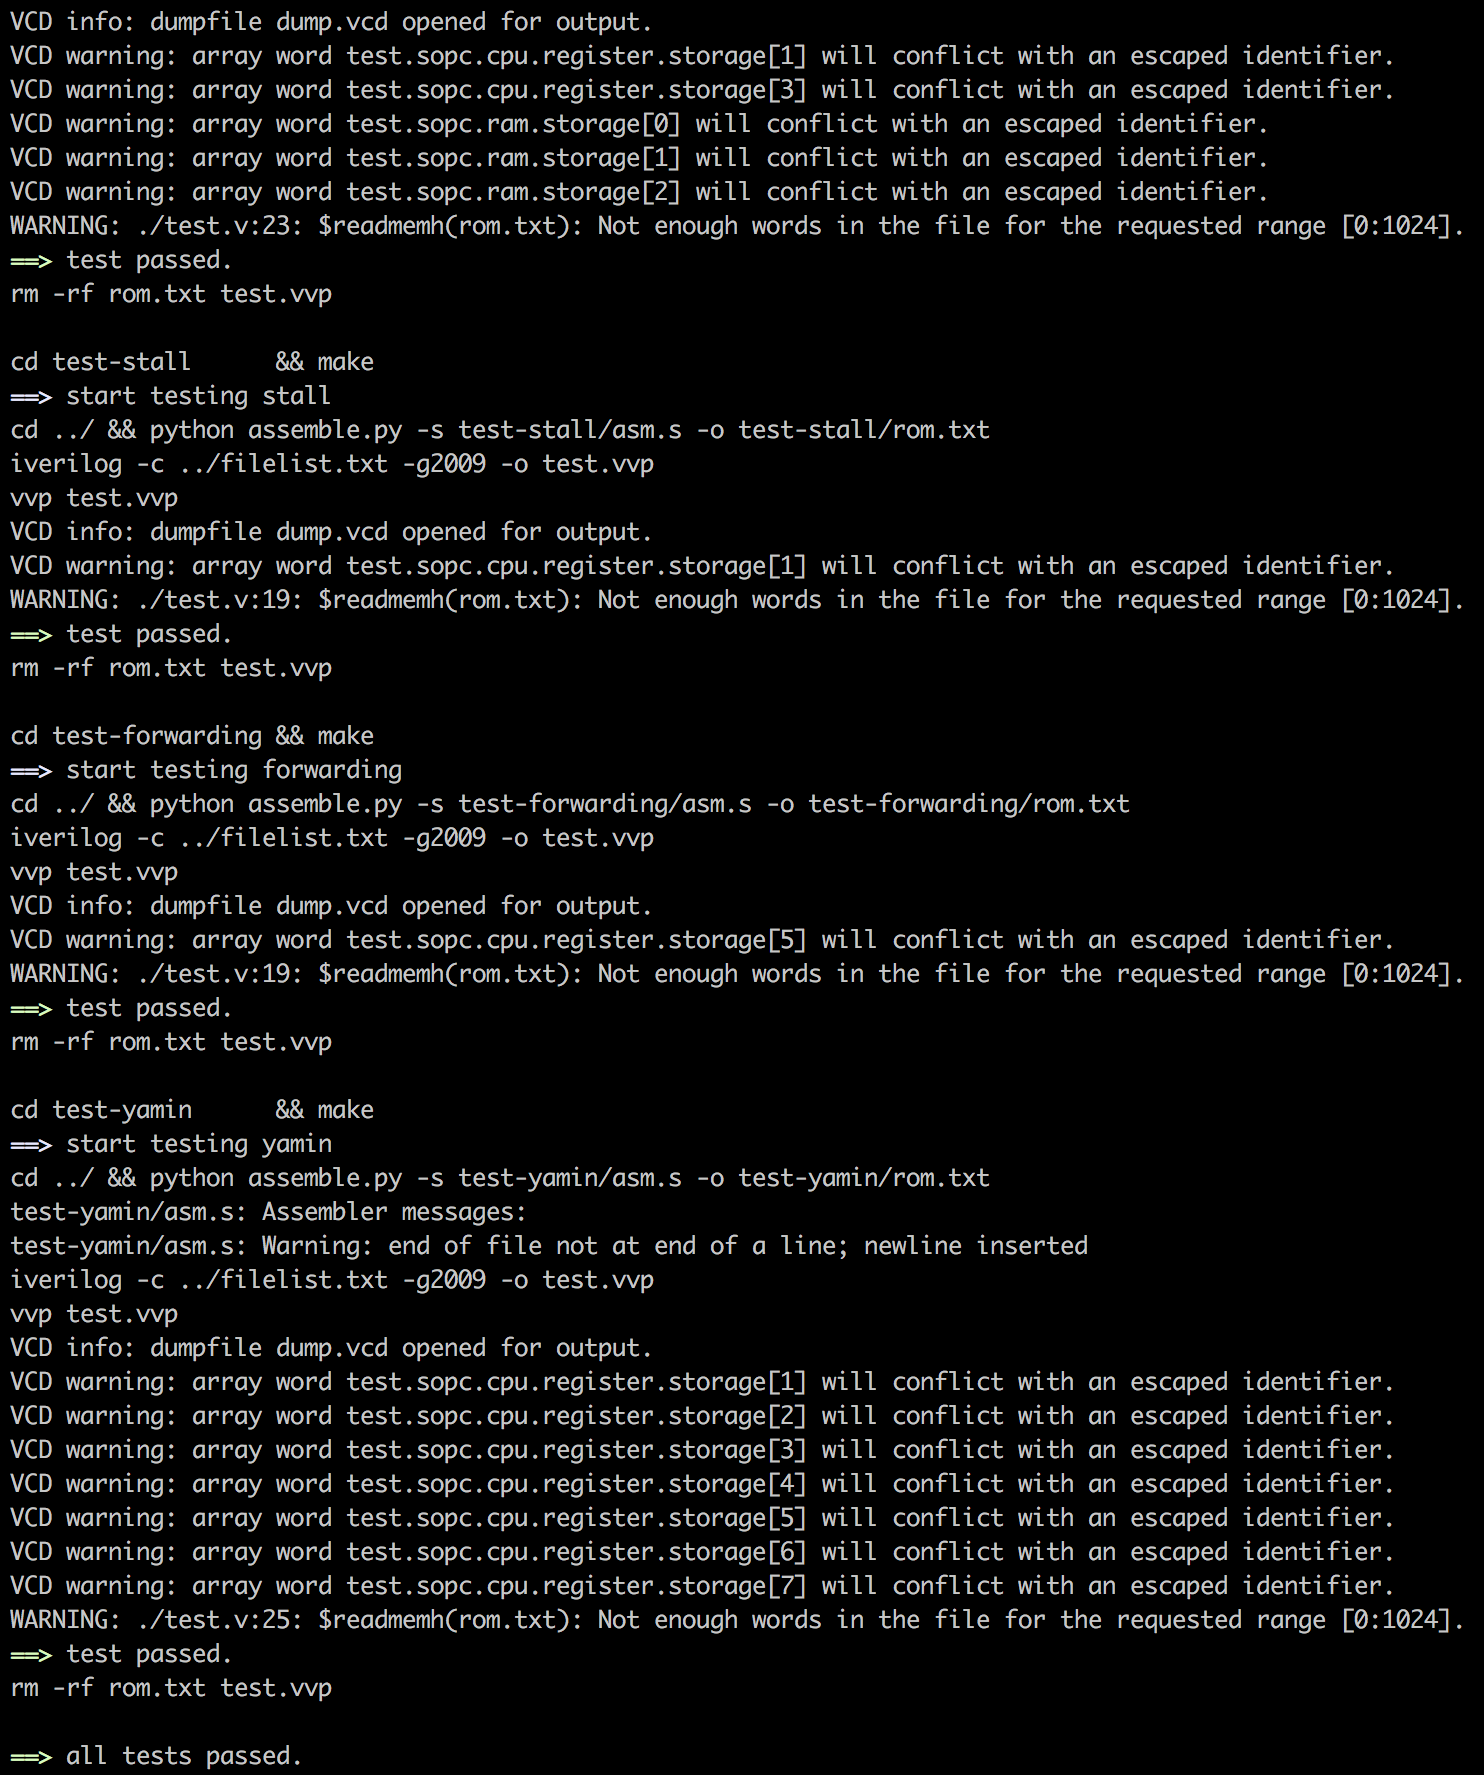
\includegraphics[width=0.9\textwidth]{image/terminal}
\caption{the automatic testing result in the terminal}
\end{center}
\end{figure}

At the meantime, a waveform simulation file (\texttt{test.vcd}) will be generated in each test case folder. Here are some waveforms captured on Scansion\footnote{\url{http://www.logicpoet.com/scansion/}}.
\begin{figure}[!h]
\begin{center}
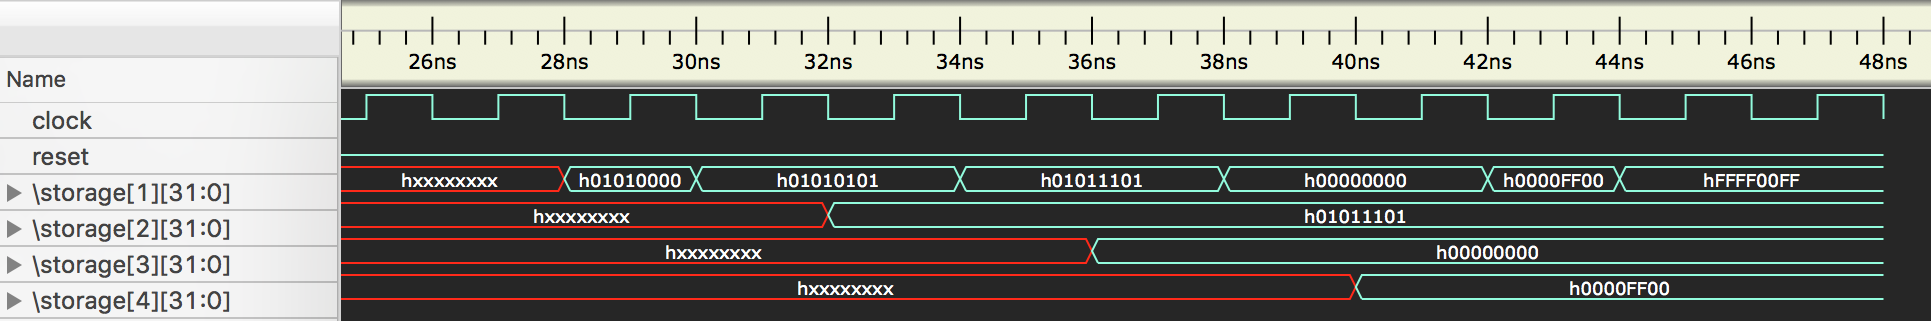
\includegraphics[width=0.9\textwidth]{image/test-logic}
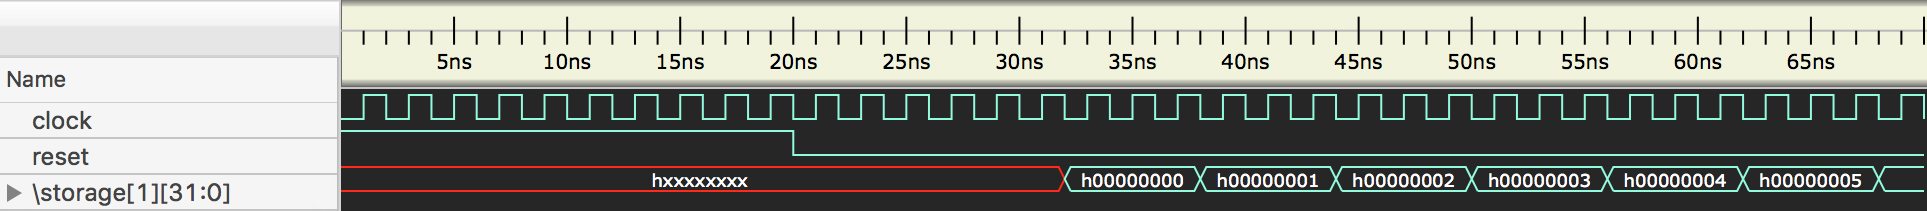
\includegraphics[width=0.9\textwidth]{image/test-jump}
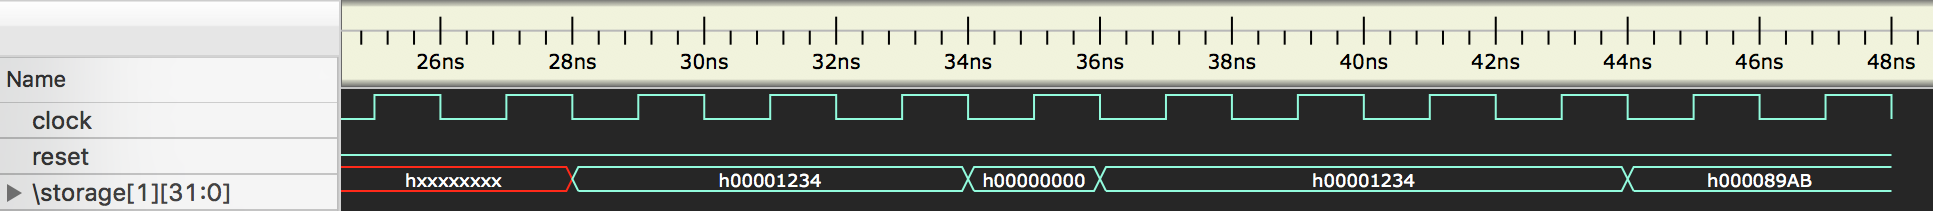
\includegraphics[width=0.9\textwidth]{image/test-stall}
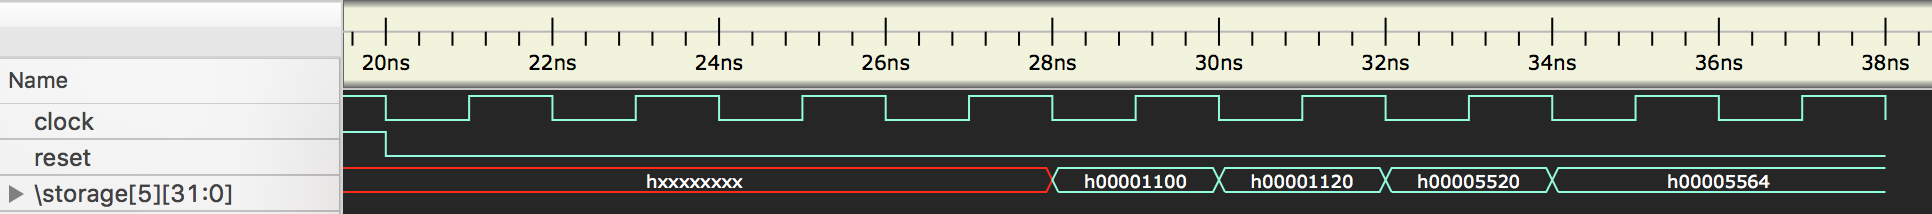
\includegraphics[width=0.9\textwidth]{image/test-forwarding}
\caption{the waveform simulation of some test cases}
\end{center}
\end{figure}

%\section{Technical Detail}
%
%\subsection{Assembler}
%
%\subsection{Automatic Test}

\section{Discussion}
Due to time constraints, it would be impossible to support all of the amazing features. As far as I know, this project has multiple aspects that can be further enhanced and refined:
\begin{itemize}
\item
Instruction cache and data cache.

There is no memory delay by now because all of the tests are functional simulation. Nevertheless, instruction cache and data cache are indispensable if we want to run this CPU on the FPGA. 
\item
Static and dynamic branch prediction.

Control hazards harm the performance badly while the static and dynamic branch prediction can mitigate the control hazards to a large extent.

In my current implementation, one delay slot is supported to help alleviate this problem. Unfortunately, this solution is not always practicable since in some cases, the compiler cannot find any codes to fill in the delay slot.
\item
Out-of-order execution with Tomasulo's algorithm\footnote{\url{https://en.wikipedia.org/wiki/Tomasulo_algorithm}}.

The major innovations of Tomasulo's algorithm include register renaming in hardware, reservation stations for all execution units, and a common data bus on which computed values broadcast to all reservation stations. These developments allow for improved parallel execution of instructions.
\item
Exception and interruption.

To run a modern operating system, the CPU should be able to handle the internal exceptions and external interruptions. In order to support these features, the coprocessor should be implemented.
\end{itemize}
I plan to support most of these features in the coming "Computer System" course.

\section{Acknowledgements}
I would like to thank Professor Alei Liang for bringing me such a wonderful course, Shusheng He for his hard work and warm devotion, and Yurong You, Zihao Ye and Lequn Chen for valuable discussions.

\newpage
\nocite{patterson2013computer, hennessy2011computer, li2011computer, palnitkar2003verilog, lei2014computer}

\bibliographystyle{apalike}
\bibliography{reference}

\end{document}